\documentclass[a4paper]{article}
\usepackage[ngerman]{babel}
\usepackage[T1]{fontenc}
\usepackage[utf8]{inputenc}
\usepackage{pdfpages}
\usepackage{a4wide}
\usepackage{amsmath}
\usepackage{amssymb}
\usepackage{graphics}
\usepackage{mathrsfs}
\usepackage{xspace}
\usepackage{verbatim}
\usepackage{float}
\usepackage{csvsimple}
\usepackage{pgfplotstable} % Generates table from .csv
\usepackage{setspace}
\usepackage{currfile}
\restylefloat{table}
\providecommand{\zB}{z.\,B.\@\xspace}
\providecommand{\Matlab}{\textsc{Matlab}\xspace}
\usepackage[binary-units]{siunitx}
\sisetup{locale = DE}
\sisetup{per-mode = symbol-or-fraction}
\DeclareSIUnit\rounds{U}
\DeclareSIUnit\nmeter{Nm}
\usepackage[breaklinks=true]{hyperref}
\renewcommand{\j}{\jmath}
% Ableitungen
\newcommand{\dd}{\mathop{}\!\mathrm{d}}
\newcommand{\Diff}[2]{\frac{\dd#1}{\dd#2}}
\newcommand{\DiffT}[1]{\Diff{#1}{t}}
\newcommand{\DDiff}[2]{\frac{\dd^2#1}{\dd#2^2}}
\newcommand{\DDiffT}[1]{\DDiff{#1}{t}}
\newcommand{\PartDiff}[2]{\frac{\partial #1}{\partial #2}}
\newcommand{\PartDiffT}[1]{\Diff{#1}{t}}
\newcommand{\PartDDiff}[2]{\frac{\partial^2 #1}{\partial #2^2}}
\newcommand{\PartDDiffT}[1]{\DDiff{#1}{t}}

% Makro für Gleichungen, Abbildungen, Tabellen
\newcommand{\abb}[1]{Abb. \ref{#1}}
\newcommand{\tab}[1]{Tab. \ref{#1}}
\newcommand{\glg}[1]{Glg. \ref{#1}}
\newcommand{\chp}[1]{Kap. \ref{#1}}
\usepackage[european]{circuitikz}
\usepackage{tikz}
\usetikzlibrary{arrows,decorations,intersections, decorations.text,calc}
\usepackage{pgfplots}
\pgfplotsset{compat=1.15}
\usepgfplotslibrary{units}
\pgfplotsset{ticklabel style={/pgf/number format/use comma,/pgf/number format/1000 sep={ }}}
\usetikzlibrary{external}
\tikzexternalize[prefix=tikz/,optimize command away=\includepdf]
\tikzset{external/up to date check=simple}
%\tikzset{external/force remake}
\definecolor{green}{HTML}{228B22}
\begin{document}
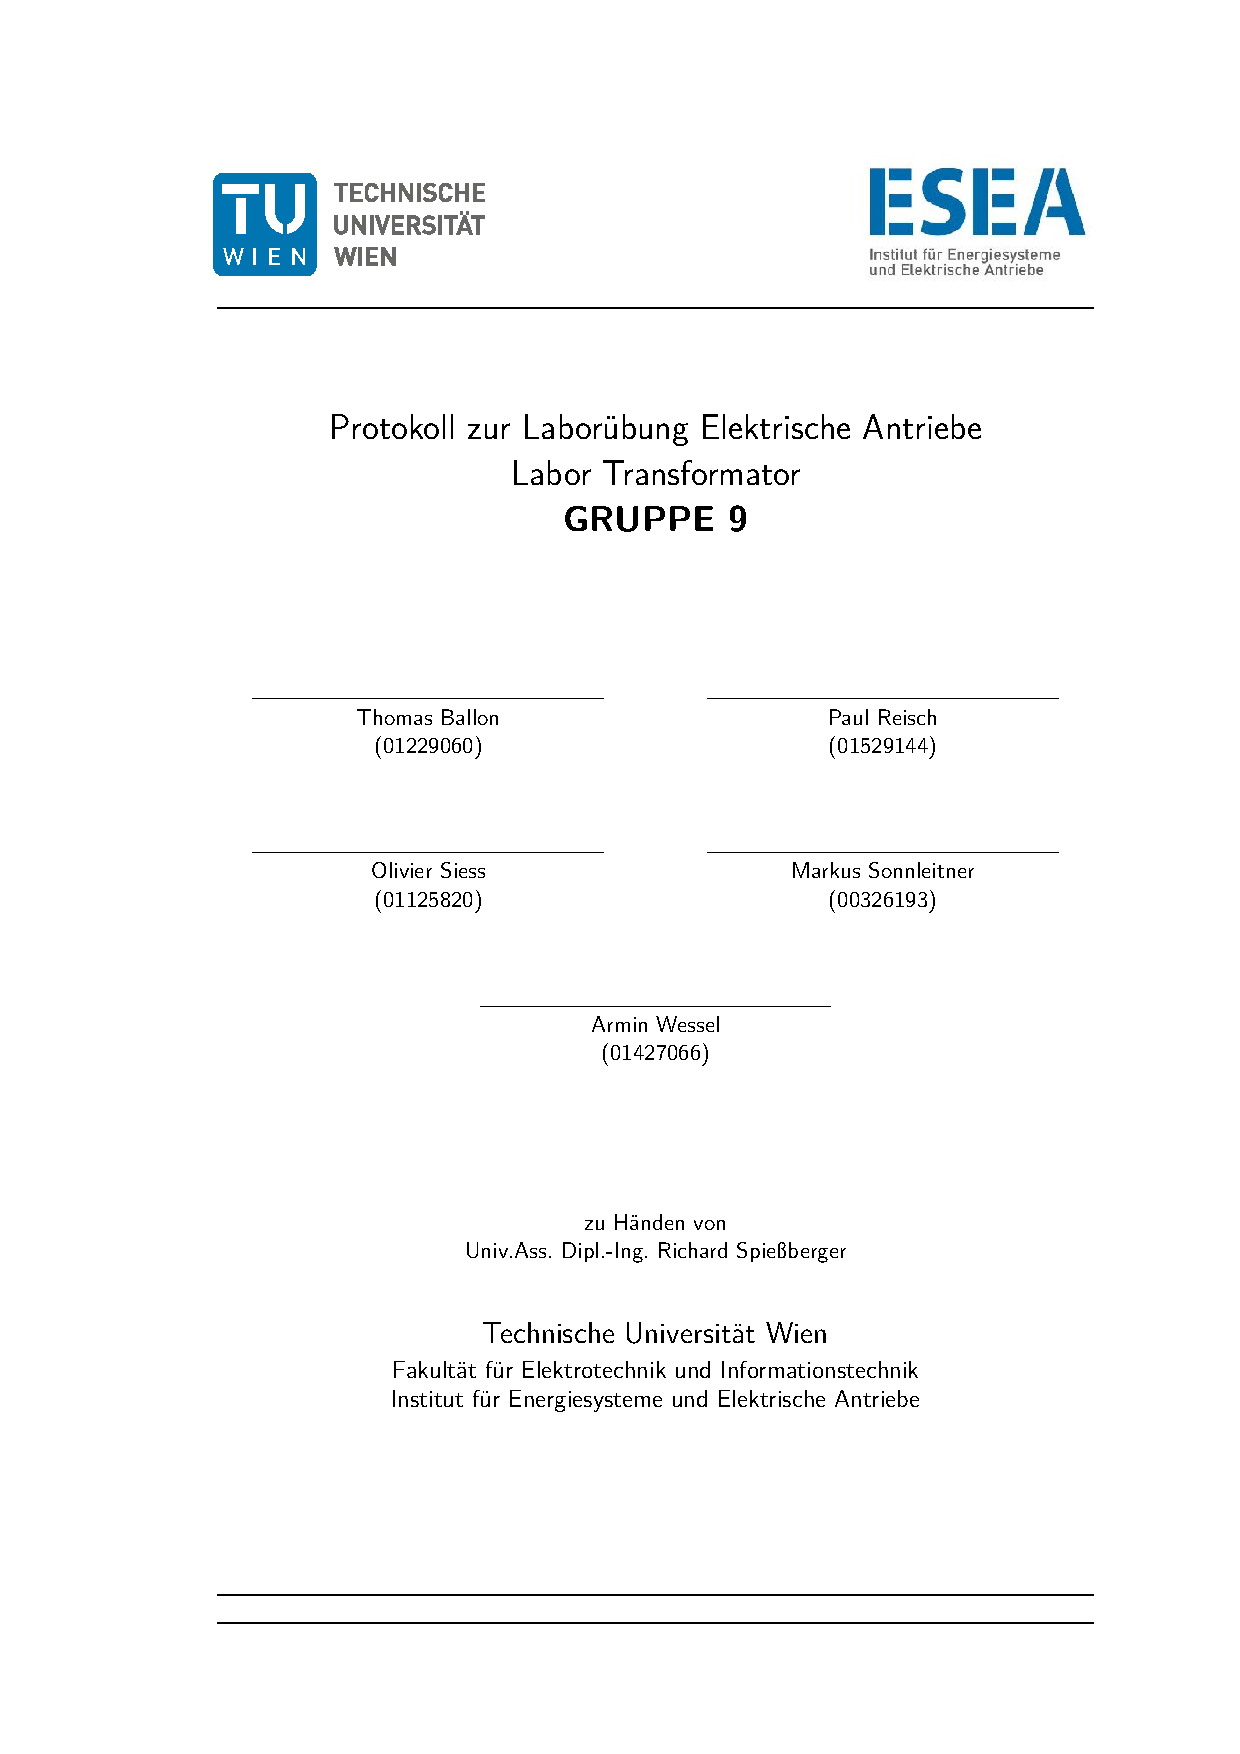
\includepdf{Deckblatt_TRAFO}
\tableofcontents\newpage
\section{Leerlaufversuch}
Der Leerlaufversuch dient der Bestimmung der Leelraufverlusten,  die aus Eisenverlusten (Hystere- und Wirbelstromverlusten), sowie Zusatzverlusten  (Streuflüsse  bei  unsym.   Bauformen)  bestehen. DIe Kupferverluste können bei dieser Messung vernachlässigt werden.\\
Für die Durchführung ist nur die Primärseite des Transformators veraschaltet, während die Sekundärseite noch nicht verschalten ist bzw. offen ist. 
Bei der Messung werden alle Außenleiterspannungen und Strangströme der Primärseite gemessen und für die Berechnungen die jeweils gemittelten Werte genutzt.
\input{\currfiledir leerlauf}
\input{\currfiledir leerlauf_spannung}
\input{\currfiledir zeitverlauf}

\section{Einschaltvorgang}

\input{\currfiledir zeitverlauf}

\section{Schaltgruppenbestimmung}\label{sec:3}
Um die Schaltgruppe zu bestimmen, musste zuerst eine Schaltgruppe gewählt werden und dann über die Anschlussklemmen auf der Sekundärseite des Trafos realisiert werden. Da die Oberspannungsseite bereits als Sternschaltung vorgegeben war, wurde als Schaltgruppe eine \textbf{Yd11} Verschaltung gewählt.\\
Da die Unterspannungswicklungen nur für eine Spannung von \SI{63.5}{\volt} ausgelegt sind, wurden vier Wicklungen pro Strang in Serie geschaltet, wobei der Bezugssinn der Spulen der Primär- und Sekundärseite für den notwendigen Durchflutungsausgleich zu beachten war. Die genaue Verschaltung kann der Abbildung \ref{fig:Verschaltung_Sekundaerseite} entnommen werden.
\begin{figure}[htb]
    \centering
    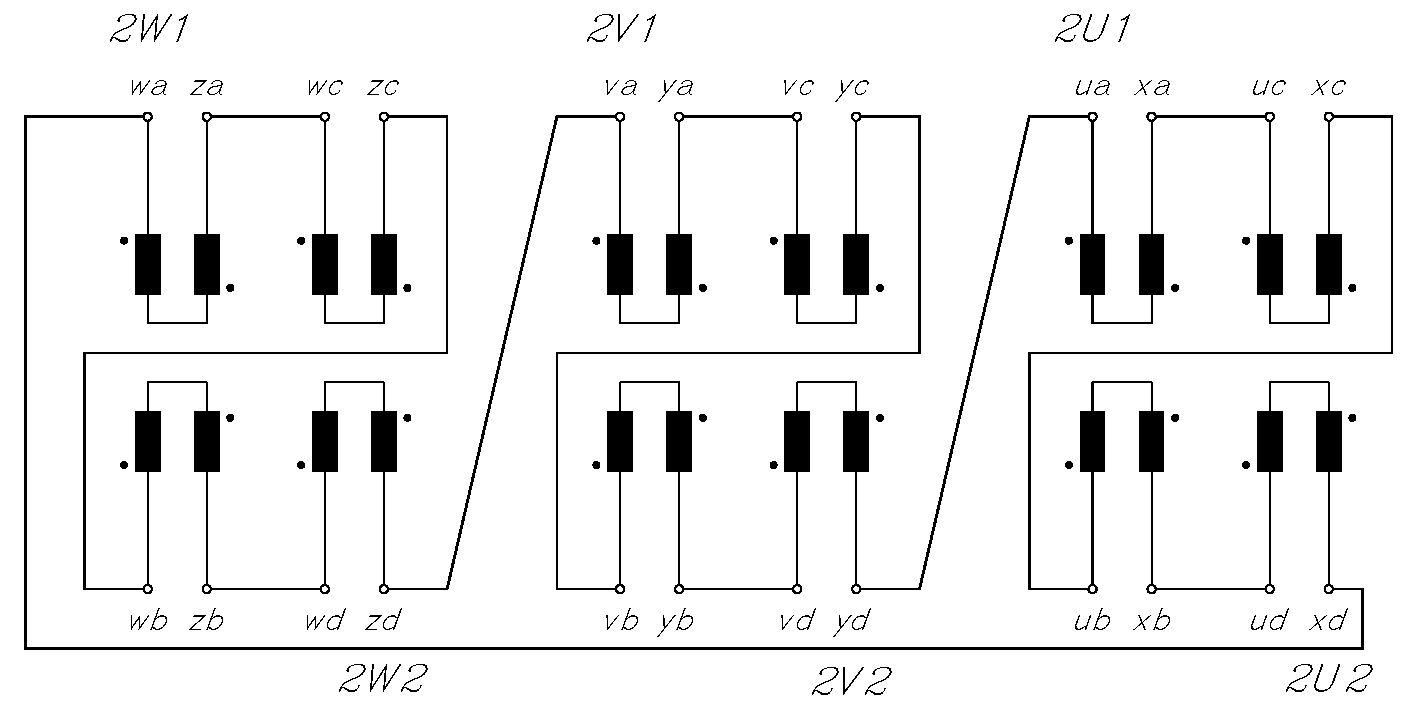
\includegraphics[width=1.0\textwidth, angle=0]{3/images/Schaltgruppe.pdf}
    \caption{Verschaltung der Sekundärwicklungen für eine Yd11 Schaltung}
    \label{fig:Verschaltung_Sekundaerseite}
\end{figure}
Die Schaltgruppenbestimmung dient der Überprüfung der Verschaltung, um sicherzustellen, dass keine Fehler gemacht wurden. Für die Messung muss Primär- und Sekundärseite auf ein gemeinsames Bezugspotential gelegt werden (für Versuchsmessungen zulässig). Dazu wurden die Punkte 1U und 2U verbunden. Die speisende Spannung wurde auf \SI{100}{\volt} begrenzt, wodurch sichergestellt wird, dass die zu messenden Spannungen im zulässigen Messbereich der verwendeten Multimeter zu liegen kommen. Die gemessenen Primär-, Sekundär- und Gegenspannungen für das dreiphasige Zeigerdiagramm (Abb. \ref{fig:schaltgruppe_messung}) sind in der nachstehenden Tabelle \ref{tab:Messwerte_Schaltgruppe} notiert. Die Messschaltung (Schaltgruppe, Messpotential 1U/2U) ist in Abbildung\;\ref{fig:Schaltgruppe_Messschaltung} dargestellt.
\begin{figure}[h!]
    \centering
    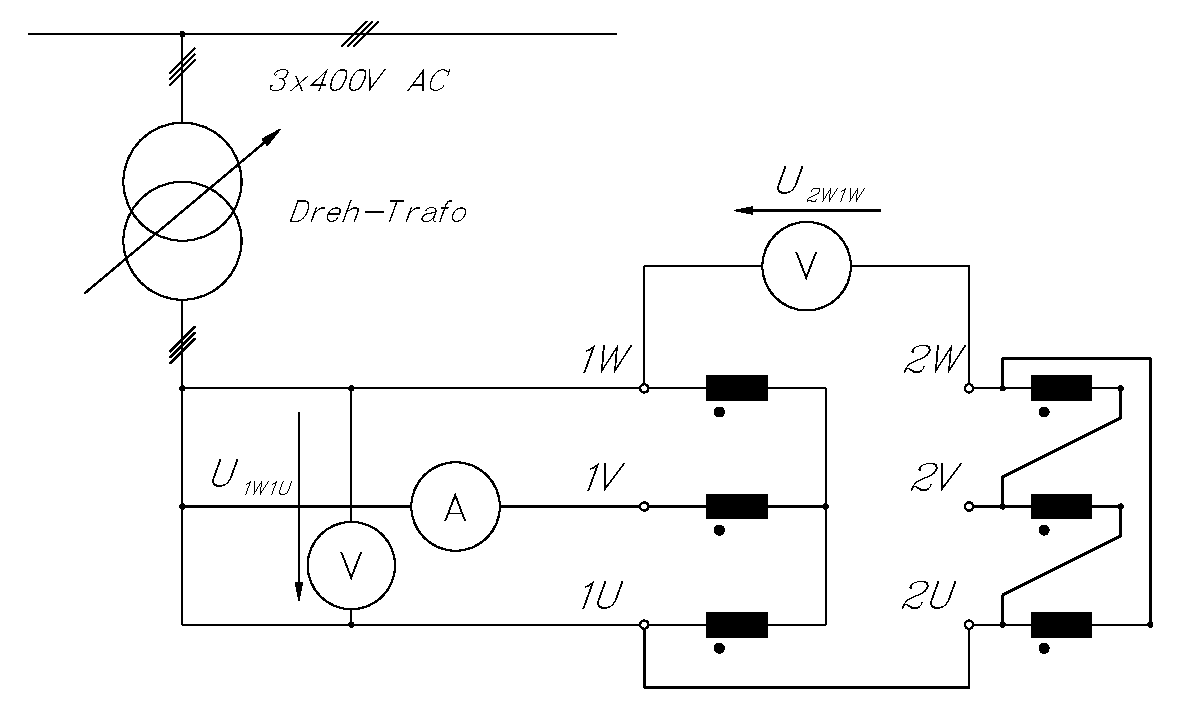
\includegraphics[width=0.75\textwidth, angle =0]{3/images/Schaltgruppe_Messungen.pdf}
    \caption{Messschaltung zur Verifikation der Schaltgruppe \textbf{Yd11}; Messungen der verschiedenen (primär-, sekundärseitigen und gegenseitigen) Spannungen (z.B.: $U_{2W1W}$).}
    \label{fig:Schaltgruppe_Messschaltung}
\end{figure}
\begin{table}[h!]
    \centering
    %\resizebox{\textwidth}{!}
    \caption{Messwerte zur Schaltgruppenbestimmung}
    \label{tab:Messwerte_Schaltgruppe}
\end{table}
Zusätzlich zur Konstruktion des Zeigerdiagramms, wird die Schaltgruppe auch durch die Verhältnisse der Windungszahlen und Spannungen der Ober- und Unterspannungsseite verifiziert.\\
Das Windungsverhältnis ergibt sich aufgrund der Beschaltung der Ober- (Parallelschaltung der 4 Wicklungen) und Unterspannungsseite (Serienschaltung der 4 Wicklungen) lt. Typenschild zu
\begin{equation}
    \Delta_N = \frac{N_{OS}}{N_{US}}=\frac{59}{4\cdot 17}=0,868.
\end{equation}
Daraus lässt sich gemeinsam mit der Schaltgruppe \textbf{Yd} die zu erwartende Spannungsübersetzung zwischen den beiden primär- und sekundärseitigen Aussenleiterspannungen $\Delta_U$ bestimmen:
\begin{equation}
    \Delta_U = \frac{U_{OS}}{U_{US}}=\sqrt{3}\cdot \Delta_N = \sqrt{3}\,\frac{59}{68}=1,503.
\end{equation}
Die gemessene Spannungsübersetzung lässt sich aus dem Verhältnis der beiden gemessenen Aussenleiterspannungen bestimmen (z.B.: zw. W-U):
\begin{equation}
    \Delta_{U,gem} = \frac{U_{1WU}}{U_{2WU}}=\frac{\SI{100}{\volt}}{\SI{66.8}{\volt}}=1,497.
\end{equation}
\input{\currfiledir Yd11}
\input{\currfiledir schaltgruppe}
\clearpage

\section{Schieflastversuch}

\section{Schieflastversuch}
Bei diesem Versuch wurde untersucht, wie sich eine unsymmetrische unterspannungsseitige Belastung auf den Betriebszustand des Transformators auswirkt (Messschaltung siehe Abbildung\;\ref{fig:Schieflast_Messschaltung}). In der Praxis treten unsymmetrische Belastungen auf, wenn ein- oder zweiphasige Verbraucher vom Transformator gespeist werden. 
\begin{figure}[ht]
    \centering
    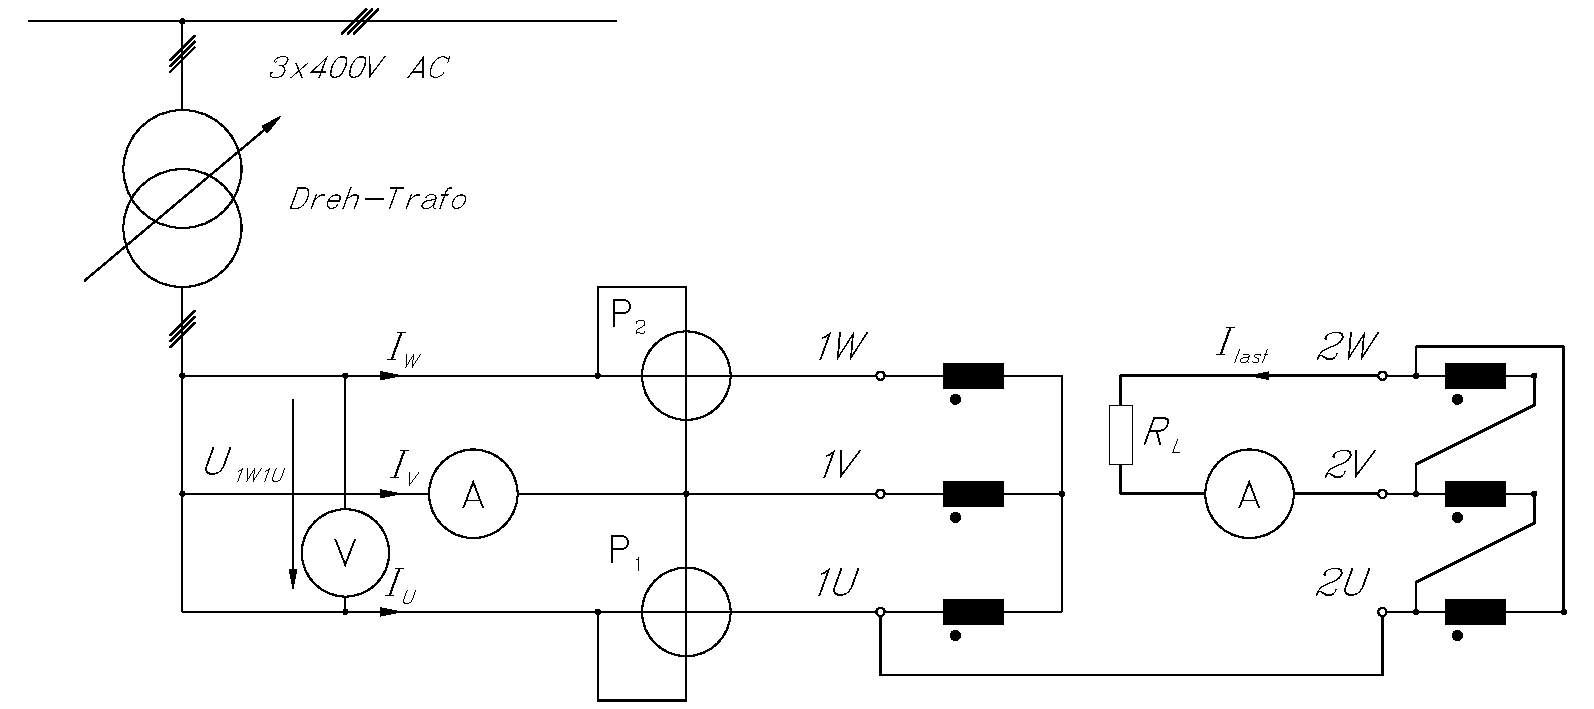
\includegraphics[width=0.75\textwidth]{\currfiledir images/Schieflast}
    \caption{Messschaltung zur Erfassung des Betriebszustandes des 3-Phasen-Transformators bei unsymmetrischer, 2-strängiger, ohmscher Belastung.}
    \label{fig:Schieflast_Messschaltung}
\end{figure}
\noindent
Für den Versuch kann im Allgemeinen entweder der Nullleiter belastet werden (einphasig, einsträngig) oder die Last zwischen zwei Außenleiter geschaltet werden (einphasig, zweisträngig). Für den Fall einer \textbf{Yd}-Schaltung ist kein sekundärseitiger Sternpunkt vorhanden, also wurde der Lastwiderstand $R_L$ zwischen zwei Außenleiter (2W - 2V) geschaltet. 

Die Dreieckwicklung in der \textbf{Yd}-Schaltung bewirkt, dass die durch unsymmetrische Belastung bedingten Nullströme als Kreisstrom auf der Sekundärseite fließen können. Dadurch ist der Durchflutungsausgleich der Schenkel gegeben. Das Primärsystem ohne angeschlossenen Sternpunktleiter muss keine Nullströme führen, und es kommt zu keiner Verzerrung der Spannungen (und keinen gleichphasigen Nullflüssen in den Schenkeln).

Der Lastwiderstand wurde so gewählt, dass näherungsweise Nennstrom fließt. An dem zur Verfügung stehendem Widerstand wurde ein Wert von $\SI{2.75}{\ohm}$ eingestellt. Das führt zu einem Strom
\begin{equation*}
    I_{Last}=\frac{\SI{253}{\volt}}{\SI{2.75}{\ohm}} = \SI{92}{\ampere},
\end{equation*}
was etwa $80\%$ des Nennstromes entspricht.
Die gemessenen Werte sind in \tab{tab:schieflast_1} angeführt.
Es wurden primärseitig die Außenleiterspannungen, die Strangströme und zwei Wirkleistungen für die 2-Wattmeter-Methode gemessen. Sekundärseitig wurde der Strom $I_{Last}$ durch den Widerstand gemessen.
\begin{table}[h!]
    \centering% Tabelle zu leerlauf.csv
    \begin{tabular}{|c|c|c|c|c|c|c|c|c|}
    \hline
    \bfseries $U_{UV}[\SI{}{\volt}]$ & \bfseries $I_U[\SI{}{\ampere}]$ & \bfseries $P_{UV}[\SI{}{\watt}]$ 
    & \bfseries $I_V[\SI{}{\ampere}]$ & \bfseries $U_{UW}[\SI{}{\volt}]$ & \bfseries $U_{WV}[\SI{}{\volt}]$ 
    & \bfseries $I_W[\SI{}{\ampere}]$ & \bfseries $P_{WV}[\SI{}{\watt}]$ & \bfseries $I_{Last}[\SI{}{\ampere}]$
    \csvreader[head to column names]{5/schieflast_1.csv}{}  
    {\\\hline\csvcoli& \csvcolii& \csvcoliii& \csvcoliv& \csvcolv& \csvcolvi& \csvcolvii& \csvcolviii& \csvcolix}
    \\\hline
    \end{tabular}
    \caption{Messwerte zum Schieflastversuch}
    \label{tab:schieflast_1}
\end{table}
\noindent Aus den gemessenen Leistungen errechnet sich die Gesamt-Wirkleistung zu
\begin{equation*}
    P_{ges}=P_{UV}+P_{WV}=\SI{21.7}{\kilo\watt}.
\end{equation*}
% Die Scheinleistung ergibt sich zu
% \begin{equation*}
%     S=
% \end{equation*}
\noindent Die gemessenen gegenseitigen Spannungen zwischen Primär- und Sekundärseite sind in \tab{tab:schieflast_2} angeführt.


\input{\currfiledir schieflast}

\begin{table}[h!]
    \centering% Tabelle zu leerlauf.csv
    \begin{tabular}{|c|c|}
    \hline
    \bfseries  $U_{1U2U}$& \bfseries $0.3$
    \csvreader[]{5/schieflast_2.csv}{}
    {\\\hline\csvcoli& \csvcolii}
    \\\hline
    \end{tabular}
    \caption{Messwerte zur Bestimmung des Zeigerdiagramms; alle Spannungen in $\SI{}{\volt}$}
    \label{tab:schieflast_2}
\end{table}
Das Zeigerdiagramm in Abb.\;\ref{fig:zeigerdiagramm_schieflast} wurde genauso konstruiert wie im Punkt \ref{sec:3}.
Der sekundärseitige Laststrom fließt aufgrund der Dreieckschaltung nur durch die Wicklung (W).
Das Verhältnis der primären Ströme ist in Abb. \ref{fig:zeigerdiagramm_pri_stroeme} dargestellt. Da an die primärseitige Sternschaltung kein Neutralleiter angeschlossen ist, muss im Sternpunkt immer die Kirchhoff'sche Knotenregel 
\begin{equation*}
    \underline{I}_U + \underline{I}_V + \underline{I}_W = 0
\end{equation*}
erfüllt sein, weshalb auf der Primärseite eine gleichartige Stromaufnahme (nur 1 Wicklung stromdurchflossen) nicht möglich ist. D.h. die Wicklungen $1U$ und $1V$ sind ebenfalls stromdurchflossen und der notwendige Durchflutungsausgleich (durch $2U$ und $2V$) wird durch einen sekundärseitigen Kreisstrom in der Dreieckswicklung ermöglicht. 

%\newpage \section{Anhang}
\begin{table}[ht!]
    \centering% Tabelle zu leerlauf.csv
    \begin{tabular}{|c|c|c|c|c|}
    \hline
    \bfseries $I_0[\SI{}{\ampere}]$ & \bfseries $P_0[\SI{}{\watt}]$ & \bfseries $S_0[\SI{}{\volt\ampere}]$ & \bfseries $U_0[\SI{}{\volt}]$ & \bfseries $\mathrm{cos}(\varphi)[\SI{}{1}]$ 
    \csvreader[head to column names]{1/leerlauf.csv}{}
    {\\\hline\csvcoli& \csvcolii& \csvcoliii& \csvcoliv& \csvcolv}
    \\\hline
    \end{tabular}
    \caption{Messwerte zum Leerlaufversuch}
    \label{tab:leerlauf}
\end{table}

\begin{table}[ht!]
    \centering% Tabelle zu kurzschluss.csv
    \begin{tabular}{|c|c|c|c|c|}
    \hline
    \bfseries $I_k[\SI{}{\ampere}]$ & \bfseries $P_k[\SI{}{\watt}]$ & \bfseries $S_k[\SI{}{\volt\ampere}]$ & \bfseries $U_k[\SI{}{\volt}]$ & \bfseries $\mathrm{cos}(\varphi)[\SI{}{1}]$
    \csvreader[head to column names]{4/kurzschluss.csv}{}
    {\\\hline\csvcoli& \csvcolii& \csvcoliii& \csvcoliv& \csvcolv}
    \\\hline
    \end{tabular}
    \caption{Messwerte zum Kurzschlussversuch}
    \label{tab:kurzschluss}
\end{table}

 brauchen wir nicht 
\end{document}
%% Link zu Laborvorbereitung und Mitschrift:
%% https://drive.google.com/file/d/1Nk3MftkeQXkkuzXWRtU5vGNyyXJULtrB/view?usp=sharing
%% https://drive.google.com/file/d/1yQ4MdQgqCzDfHTdPBfUZE8cH-W7nPDpl/view?usp=sharing